\documentclass[12pt]{article}
\usepackage{graphicx}
\usepackage{subfig}
\newcommand\mytab{\tab \hspace{+1cm}}
\usepackage{fancyhdr}
\usepackage{enumitem}
\usepackage{tikz-cd}
\usepackage{geometry}
\usepackage{tikz}
\usepackage{tikz,lipsum,lmodern}
\DeclareMathAlphabet{\mathcal}{OMS}{cmsy}{m}{n}
\usepackage[most]{tcolorbox}
 \geometry{
 a4paper,
 total={170mm,257mm},
 left=20mm,
 top=20mm,
 }
\usepackage[utf8]{inputenc}
\linespread{1.2}
\usepackage{tikz,lipsum,lmodern}
\usepackage{hyperref}
\newtcolorbox{mybox}{
enhanced,
boxrule=0pt,frame hidden,
borderline west={4pt}{0pt}{green!75!black},
colback=green!10!white,
sharp corners
}
\newtcolorbox{mybox2}{
enhanced,
boxrule=0pt,frame hidden,
borderline west={4pt}{0pt}{blue!75!black},
colback=blue!10!white,
sharp corners
}
\usepackage{amsmath,amsfonts,amsthm,bm} % Math packages
\usepackage[most]{tcolorbox}
\usepackage{amssymb}
\hypersetup{
    colorlinks=true,
    linkcolor=blue,
    filecolor=magenta,      
    urlcolor=cyan,
    pdftitle={Overleaf Example},
    pdfpagemode=FullScreen,
    }
\usepackage{amsmath}

\usepackage{natbib}
\usepackage{wrapfig}
\usepackage{mathtools}
\usepackage{url}
\usepackage{pax}
\usepackage{pdfpages}
\usepackage{graphicx}
\usepackage{mathptmx}
\usepackage{tikz}
\usepackage{blindtext}
\title{MA2104 AY24/25 Sem 2 Final}
\author{
  Solution by Malcolm Tan Jun Xi\\
  Audited by Thang Pang Ern
}
\date{}


\begin{document}

\maketitle
\noindent\textbf{Question 1:} Let
\begin{align*}
    f(x,y,z)=z\sqrt{x^2+y^2}
\end{align*}
Let $E$ be the solid which is bounded by two cylinders $x^2+y^2=1$ and $x^2+y^2=4$ and two planes $z=0$ and $z=6$. Evaluate
\begin{align*}
    \iiint_E f(x,y,z)\ dV
\end{align*}
\emph{Solution:} By considering cylindrical coordinates, we let
\begin{align*}
    x=r\cos\theta,\qquad y=r\sin\theta,\qquad z=z
\end{align*}
such that we have
\begin{align*}
    \iiint_E f(x,y,z)&=\int_0^{2\pi}\int_1^2\int_0^6 zr^2\ dzdrd\theta\\
    &=84\pi
\end{align*}\qed\\[2em]
\textbf{Question 2:} Consider the surface
\begin{align*}
    S:=\{(x,y,z)\in\mathbb{R}^3\ |\ z^2=x^2+y^2, 1\leq z\leq 3 \}
\end{align*}
which is part of the cone $z^2=x^2+y^2$ between $z=1$ and $z=3$. Let
\begin{align*}
    f(x,y,z)=e^{-x^2-y^2}
\end{align*}
Evaluate
\begin{align*}
    \iint_S f(x,y,z)\ dS
\end{align*}\\[2em]
\emph{Solution:}  By considering cylindrical coordinates, we let
\begin{align*}
    x=r\cos\theta,\qquad y=r\sin\theta,\qquad z=r
\end{align*}
such that we have
\begin{align*}
    \textbf{r}(r,\theta)=(r\cos\theta,r\sin\theta,r)
\end{align*}
By Jacobian transformation, we have
\begin{align*}
    dS=\left|\textbf{r}_r(r,\theta)\times \textbf{r}_\theta(r,\theta)\right|drd\theta=\sqrt{2}r\ drd\theta
\end{align*}
Hence
\begin{align*}
    \iint_Sf(x,y,z)\ dS&=\int_0^{2\pi}\int_1^3e^{-r^2}\cdot \sqrt{2}r\ drd\theta\\
    &=\sqrt{2}\pi(e^{-1}-e^{-9})
\end{align*}\qed\\[2em]
\textbf{Question 3:}
\begin{enumerate}[label=\alph*)]
    \item Let $C_1$ be the positively oriented closed curve consisting of the upper half of the unit circle from $(-1,0)$ to $(1,0)$, and the line segments from $(1,0)$ to $(2,0)$, from $(2,0)$ to $(2,2)$, from $(2,2)$ to $(-2,2)$, from $(-2,2)$ to $(-2,0)$ and from $(-2,0)$ to $(-1,0)$. Evaluate
    \begin{align*}
        \int_{C_1} y(\cos x-1)\ dx+\sin x\ dy
    \end{align*}
    \item Recall that for a curve $C$ with position vector $\textbf{r}$, denote $d\textbf{r}=\textbf{T}ds$ where \textbf{T} is the unit tangent vector (with the given orientation) at a point of $C$. Let $\textbf{F}(x,y)=\langle \frac{-y}{x^2+y^2},\frac{x}{x^2+y^2}\rangle$. Let $C_2$ be the unit circle which is positively oriented (i.e. anticlockwise), and let $C_3$ be the positively oriented ellipse $\{(x,y)\in\mathbb{R}^2\ |\ \frac{x^2}{4}+\frac{y^2}{9}=1\}$. Evaluate
    \begin{align*}
        \int_{C_2} \textbf{F}.d\textbf{r}\quad\text{and}\quad \int_{C_2}\textbf{F}.d\textbf{r}
    \end{align*}\\[2em]
    \emph{Solution:}\\
    (a) By Green's Theorem, we have
    \begin{align*}
        \int_{C_1} y(\cos x-1)\ dx+\sin x\ dy=\iint \cos x-(\cos x-1)\ dA=\iint dA=\text{Area of }C_1
    \end{align*}
\end{enumerate}
\begin{center}
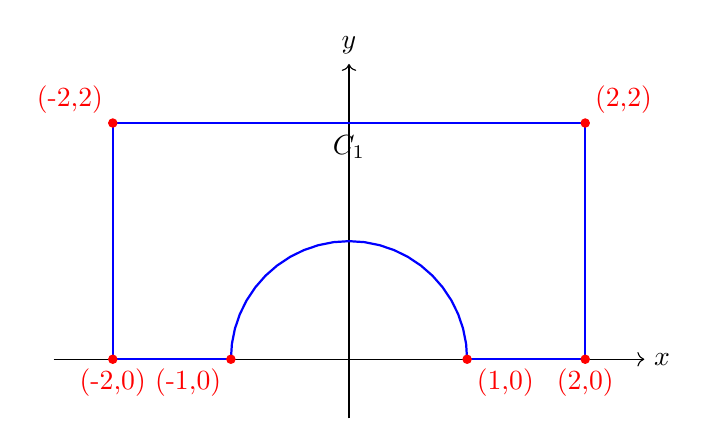
\begin{tikzpicture}[scale=1.5]
    % Axes
    \draw[->] (-2.5,0) -- (2.5,0) node[right] {$x$};
    \draw[->] (0,-0.5) -- (0,2.5) node[above] {$y$};

    % Upper half of the unit circle from (-1,0) to (1,0)
    \draw[thick, blue, domain=180:0] plot ({cos(\x)}, {sin(\x)});

    % Line segments forming the rest of the curve
    \draw[thick, blue] (1,0) -- (2,0) -- (2,2) -- (-2,2) -- (-2,0) -- (-1,0);

    % Points
    \filldraw[red] (-1,0) circle (1pt) node[below left] {(-1,0)};
    \filldraw[red] (1,0) circle (1pt) node[below right] {(1,0)};
    \filldraw[red] (2,0) circle (1pt) node[below] {(2,0)};
    \filldraw[red] (2,2) circle (1pt) node[above right] {(2,2)};
    \filldraw[red] (-2,2) circle (1pt) node[above left] {(-2,2)};
    \filldraw[red] (-2,0) circle (1pt) node[below] {(-2,0)};

    % Label
    \node at (0,1.8) {$C_1$};
\end{tikzpicture}
\end{center}
As such we have
\begin{align*}
     \int_{C_1} y(\cos x-1)\ dx+\sin x\ dy=(2)(4)-\frac{1}{2}\pi(1)^2=8-\frac{\pi}{2}
\end{align*}\qed\\[2em]
(b) Note that \textbf{F} is not defined at it origin which lies inside the circle. Therefore Green's Theorem cannot be applied here. Let
\begin{align*}
    \textbf{r}(t)=\langle\cos t,\sin t\rangle
\end{align*}
then
\begin{align*}
    \textbf{F}(\textbf{r}(t))=\langle-\sin t,\cos t\rangle\qquad\text{and}\qquad \textbf{r}'(t)= \langle-\sin t,\cos t\rangle
\end{align*}
As such 
\begin{align*}
    \int_{C_2}\textbf{F}.d\textbf{r}=\int_0^{2\pi}\langle-\sin t,\cos t\rangle\cdot\langle-\sin t,\cos t\rangle\ dt=\int_0^{2\pi}dt=2\pi
\end{align*}
(b) Similarly as (a). \textbf{F} is not defined at it origin which lies inside the circle. Therefore Green's Theorem cannot be applied here. Some may opt to parametrize the vector and will end up having
\begin{align*}
    \int_0^{2\pi} \frac{6}{4\cos^2 t+9\sin^2 t}\ dt
\end{align*}
which is messy. Instead, we can observe that 
\begin{align*}
    |\textbf{F}|=\frac{1}{r}
\end{align*}
Hence it form a closed loops around the origin, the circulation around any simple closed curve enclosing the origin exactly once and oriented clockwise is $2\pi$. Hence
\begin{align*}
    \int_{C_3}\textbf{F}.d\textbf{r}=2\pi
\end{align*}\qed\\[2em]
\textbf{Question 4:} Recall that for a surface $S$, denote $d\textbf{S}=\textbf{n}\ dS$ where $\textbf{n}$ is the unit normal vector (with the given orientation) at a point of $S$; for a curve $C$ with position vector \textbf{r}, denote $d\textbf{r}=\textbf{T}\ ds$ where \textbf{T} is the unit tangent (with the given orientation) at a point of $C$. Let $\textbf{F}(x,y,z)=\langle z^2,-2x,y^5\rangle$
\begin{enumerate}[label=\alph*)]
    \item Calculate $\operatorname{curl }\textbf{F}$
    \item Let $S_1:=\{(x,y,0)\in\mathbb{R}^3\ |\ x^2+y^2\leq 1\}$ be the unit disk in the $xy-$plane of $\mathbb{R}^3$, which is upward pointing. Calculate
    \begin{align*}
        \iint_{S_1}\operatorname{curl }\textbf{F}.d\textbf{S}
    \end{align*}
    \item Let $C_1:=\{(x,y,0)\in\mathbb{R}^3\ |\ x^2+y^2=1\}$ be the positively oriented (i.e. anticlockwise) unit circle in the $xy-$plane of $\mathbb{R}^3$. Calculate
    \begin{align*}
        \int_{C_1}\textbf{F}.d\textbf{r}
    \end{align*}
    \item Let $S_2:=\{(x,y,z)\in\mathbb{R}^3\ |\ z\geq 0, x^2+y^2+z^2=1\}$ be the upper half of the unit sphere which is positively oriented (i.e. outward pointing). Calculate
    \begin{align*}
        \iint_{S_2} \operatorname{curl }\textbf{F}.d\textbf{S}
    \end{align*}
    \item Let $\textbf{G}(x,y,z)=\langle U,V,W\rangle$ where $U,V,W$ have continuous partial derivatives in an open set $D\subset\mathbb{R}^3$. If $\textbf{G}(x,y,z)=\nabla(H(x,y,z))$ for a function $H(x,y,z)$ defined in $D$, is it true that $\operatorname{curl }\textbf{G}=\langle 0,0,0\rangle$? (Justify your answer). Conversely, if $\operatorname{curl}\textbf{G}=\langle0,0,0\rangle$ at every point in $D$, is it true that $\textbf{G}=\nabla H(x,y,z)$ for some function $H$ in the open set $D$?(No justification is needed)
\end{enumerate}
\emph{Solution:}\\
(a) It is straight forward that
\begin{align*}
    \operatorname{curl \textbf{F}}=\nabla\times \textbf{F}=\langle 5y^4,-2z,-2\rangle
\end{align*}\qed\\[2em]
(b) Since $S_1$ lies in $xy-$plane with upward normal, then
\begin{align*}
    \textbf{n}=\langle 0,0,1\rangle
\end{align*}
as such
\begin{align*}
    \iint_{S_1}\operatorname{curl }\textbf{F}.d\textbf{S}=-2\iint dA=-2\pi
\end{align*}
(c) By Stokes' Theorem,
\begin{align*}
     \int_{C_1}\textbf{F}.d\textbf{r}= \iint_{S_1}\operatorname{curl }\textbf{F}.d\textbf{S}=-2\pi
\end{align*}\qed\\[2em]
(d) Let $C_2$ be the boundary of $S_2$. By Stokes' Theorem,
\begin{align*}
    \iint_{S_2}\operatorname{curl }\textbf{F}.d\textbf{S}=\int_{C_2}\textbf{F}.d\textbf{r}
\end{align*}
At $z=0$, $x^2+y^2=1$ which is the same circle as $C_1$. Therefore
\begin{align*}
      \iint_{S_2}\operatorname{curl }\textbf{F}.d\textbf{S}=-2\pi
\end{align*}\qed\\[2em]
(e) Suppose $\textbf{G}(x,y,z)=\nabla(H(x,y,z))$, then $\textbf{G}$ is conservative. Hence it is true that $\operatorname{curl }\textbf{G}=\langle 0,0,0\rangle$. Conversely it is false as the domain needs to be simply connected but the context does not mention that the domain is simply connected Hence it is not necessarily true.\qed\\[2em]
\textbf{Question 5:} Let $\textbf{F}(x,y,z)=\frac{\langle x,y,z\rangle}{(x^2+y^2+z^2)^{\frac{3}{2}}}$
\begin{enumerate}[label=\alph*)]
    \item calculate $\operatorname{div \textbf{F}}$
    \item Let $S_a:=\{(x,y,z)\in\mathbb{R}^3\ |\ x^2+y^2+z^2=a^2\}$ be the sphere of radius $a>0$ which is positively oriented (i.e outward pointing). Calculate $\iint_{S_a}\textbf{F}.d\textbf{S}$ [N.B you may use, without proof, the fact that the sphere $S_a$ has area $4\pi a^2$]
    \item Let $S$ be the positively oriented surface which is bounded above by the paraboloid $z=1-x^2-y^2$ and is bounded below by the paraboloid $z=-1+x^2+y^2$. Calculate $\iint_S \textbf{F}.d\textbf{S}$
\end{enumerate}
\emph{Solution:} \\
(a) We have
\begin{align*}
    \operatorname{div} \textbf{F}&=\frac{x^2+y^2+z^2-3x^2}{\sqrt{(x^2+y^2+z^2)^5}}+\frac{x^2+y^2+z^2-3y^2}{\sqrt{(x^2+y^2+z^2)^5}}+\frac{x^2+y^2+z^2-3z^2}{\sqrt{(x^2+y^2+z^2)^5}}\\
    &=0
\end{align*}
(b) Note that since $\textbf{F}(x,y,z)$ is not defined at $(0,0,0)$, divergence theorem cannot be directly applied. Consider
\begin{align*}
    \textbf{n}=\frac{1}{a}\langle x,y,z\rangle
\end{align*}
As such
\begin{align*}
    \iint_{S_a}\textbf{F}.d\textbf{S}=\iint_{S_a}\frac{\textbf{r}}{a^3}\cdot \frac{\textbf{r}}{a}\ dS=\iint_{S_a}\frac{|\textbf{r}|^2}{a^4}\ d S=\frac{1}{a^2}\iint_{S_a}dS=4\pi
\end{align*}\qed\\[2em]
(c) From (b) we know that $\iint_{S_a}\textbf{F}.dS$ is independent of the radies $a$. Therefore
\begin{align*}
    \iint_S \textbf{F}.d\textbf{S}=4\pi
\end{align*}\qed
\end{document}
